\documentclass[twocolumn]{revtex4-1}
\usepackage{amsmath}
\usepackage{mathtools}
\usepackage{xcolor}
\newcommand{\lucas}[1]{\textbf{\textcolor{blue}{LKW: #1}}}
\newcommand{\shivesh}[1]{\textbf{\textcolor{purple}{SP: #1}}}


\begin{document}
\title{A light weight regularization for wave function parameter gradients
\\ in quantum Monte Carlo}

\author{Shivesh Pathak}
\email[]{sapatha2@illinois.edu}

\author{Lucas K. Wagner}
\email[]{lkwagner@illinois.edu}
\affiliation{Department of Physics; University of Illinois at Urbana-Champaign}

\date{\today}
\begin{abstract}
The parameter derivative of the expectation value of the energy, $\partial E/\partial p$, is a key ingredient in variational quantum Monte Carlo (VMC) wave function optimization methods.
A naive Monte Carlo estimate of this derivative suffers from an infinite variance which inhibits the efficiency of optimization methods that rely on a stable estimate of the derivative.
In this work, we derive a simple regularization of the naive estimator which is trivial to implement in existing VMC codes, has finite variance, and a negligible bias which can be extrapolated to zero bias with no extra cost.
We use this estimator to construct an unbiased, finite variance estimation of $\partial E/\partial p$ for a multi-Slater-Jastrow trial wave function on the LiH molecule.
As such, this regularized estimator stands stands as a light weight option for stable estimation of $\partial E/\partial p$ in VMC optimization techniques.
\end{abstract}
\maketitle 

\section{Introduction}

\lucas{Typically equations are referenced as Eqn~\ref{eq:convergent_integral}; you've done something else here. } 
\shivesh{Done.}

Accurate and stable stochastic estimation of the parameter gradient of the energy expectation value, $\partial E/\partial p$,\lucas{define $p$. In general, I think you may need to build this up a little more and explain the problem.} is an integral component of variational Monte Carlo (VMC) wave function energy optimization techniques \cite{PhysRevB.64.024512, doi:10.1063/1.1604379, Toulouse2007, Umrigar2005, Umrigar2007, Toulouse2008}.
Within these techniques, wave function parameters are updated iteratively, with the estimate of $\partial E/\partial p$ used in determining updates.
If the estimation is inaccurate, having a large bias, the final converged wave function is not guaranteed to be the lowest energy wave function in the parameterization space.
If the estimation is unstable, having a large variance, the updates will have large statistical fluctuations, decreasing efficiency.
An appropriate estimator for $\partial E/ \partial p$ should then have both low bias and variance.

A useful starting point is the naive Monte Carlo estimator for $\partial E/\partial p$ evaluated on a wave function $\Psi(\vec{p}, \vec{R})$ 
\begin{equation}
\begin{split}
\hat{\theta} \equiv \left\langle E_L(R) \frac{\partial_p \Psi(R)}{\Psi(R)} \right\rangle - \left\langle E_L(R) \right \rangle \left \langle \frac{\partial_p \Psi(R)}{\Psi(R)}\right\rangle 
\end{split}
\label{eq:naive_estimator}
\end{equation}
\lucas{My initial impression is that this feels heavy for the introduction. We should write a simpler thing, or just save the equations for later.}
The brackets $\langle \ \rangle$ are Monte Carlo expectation values over $M$ configurations drawn from the distribution $|\Psi(\vec{p}, \vec{R})|^2$, and $E_L = (\hat{H}\Psi)/\Psi$ is the local energy with Hamiltonian operator $\hat{H}$.
While unbiased, $\hat{\theta}$ has a divergent variance \cite{Avella, doi:10.1063/1.4933112} due to the behavior of the first term in Eqn~\ref{eq:naive_estimator} near the nodes of $\Psi$.
This infinite variance leads to inefficient optimization and has prompted a search for zero bias, finite variance estimators of $\partial E/\partial p$.

Current zero bias, finite variance estimation techniques were adapted from the low-variance estimation of forces in QMC \cite{doi:10.1063/1.462059, doi:10.1063/1.3516208, Phys2016} and involve guiding or auxiliary wave functions, such as a reweighting scheme \cite{Avella, Attaccalite2008, Zen2013} or improved estimators \cite{Assaraf1999, doi:10.1063/1.1286598, Assaraf2003}.
While zero bias is achieved for arbitrary guiding wave functions $\Psi_G$, finite variance is only acquired with specially tuned guiding functions which cancel the divergences in Eqn~\ref{eq:naive_estimator} near the nodes of $\Psi$.
A general form for $\Psi_G$ which yields a finite-variance estimate of $\partial E/\partial p$ is provided by Umrigar \cite{doi:10.1063/1.4933112} where $\Psi_G$ differs from $\Psi$ only near the nodes, the prior having a finite value.
Still unresolved is a zero bias, finite variance estimator for Eqn~\ref{eq:naive_estimator} without the luggage of a guiding wave function. 
\lucas{"without the luggage" is not too convincing. Isn't the point that the guiding wave function doesn't need to be tuned, and that the algorithm can be simpler?}

We derive and test a simple regularized estimator for $\partial E/\partial p$ which has finite variance, can be extrapolated to zero bias, and does not rely on guiding wave functions.
Instead, the divergence in the first term of Eqn~\ref{eq:naive_estimator} is suppressed via multiplication by a polynomial function within a distance $\epsilon$ of the nodes of $\Psi(\vec{p}, \vec{R})$. 
We present rigorous mathematical proofs for the scalings of the variance and bias of the regularized estimator with $\epsilon$, and provide an algorithm for the zero bias extrapolation of the estimate.
The mathematical predictions and extrapolation procedure are then tested in evaluating $\partial E/\partial p$ for a multi-Slater-Jastrow (MSJ) trial wave function on the LiH molecule.

\section{Regularized estimator}
The naive estimator Eqn~\ref{eq:naive_estimator} suffers from an infinite variance. 
\lucas{Should explain the na\"ive estimator here in a little more detail. } 
The divergent contribution to the variance arises from the evaluation of the integral
\begin{equation}
\int \Big(E_L\frac{\partial_p\Psi}{\Psi}\Big)^2 |\Psi|^2 dR.
\label{eq:divergent_integral}
\end{equation}
when $\Psi$ is not an eigenstate of $\hat{H}$ and the parameter $p$ affects the nodes of $\Psi$, such as orbital or determinantal coefficients.
In this case, to lowest order in distance $|\vec{R}-\vec{N}|$ from a nodal point $\vec{N}$ of $\Psi$, $\hat{H}\Psi$ and $\partial_p \Psi \sim const$ and $\Psi \sim \nabla \Psi(\vec{N}) \cdot (\vec{R} - \vec{N})$, leading to the integrand in Eqn~\ref{eq:divergent_integral} behaving as $1/|\vec{R}-\vec{N}|^2$ near the node.
Since the integration domain includes the nodal surface of $\Psi$, the $1/|\vec{R}-\vec{N}|^2$ behavior of the integrand as $|\vec{R}-\vec{N}|\rightarrow 0$ leads to a divergent integral.

We obtain a finite variance estimator for $\partial E/\partial p$ by multiplying the first term in the naive estimator Eqn~\ref{eq:naive_estimator} by a function $f_\epsilon$:
\begin{equation}
\begin{split}
&\hat{\theta_\epsilon} \equiv \\ 
&\left\langle E_L(R) \frac{\partial_p \Psi(R)}{\Psi(R)} f_\epsilon(R) \right\rangle - \left\langle E_L(R) \right \rangle \left \langle \frac{\partial_p \Psi(R)}{\Psi(R)} f_\epsilon(R) \right\rangle
\label{eq:regularized_estimator}
\end{split}
\end{equation}
\lucas{the notation with all the summations is not very easy to read to me. Typically we would say something like $\left\langle E_L(R) \frac{\partial_p \Psi(R)}{\Psi(R)} f_\epsilon(R) \right\rangle_{R\sim\Psi_T^2}$. Also, is the second expectation value also regularlized? Why not?}
\shivesh{Updated the summations. The second term does need to be regularized, added that in}.
where 
\begin{equation}
f_\epsilon(\vec{R}) = \begin{cases} 
      \sum_{l=n}^{\infty} a_l |\frac{\vec{x}}{\epsilon}|^n & |\frac{\vec{x}}{\epsilon}| < 1 \\
      1 & |\frac{\vec{x}}{\epsilon}| \ge 1 \\
   \end{cases},\ \vec{x} \equiv \frac{\nabla \Psi(\vec{R}) \Psi(\vec{R})}{|\nabla \Psi(\vec{R})|^2},
\label{eq:regularizing_function}
\end{equation} 
where the constants $a_n$ can take any real value.
\lucas{What does the O notation mean here? This is not explained? If it's meant to be big-O notation, that uses $\mathcal{O}$, and it shouldn't be used here. Just say that it's proportional to.} 
\shivesh{Updated to remove any O and just explicitly write down the general form of $f_\epsilon$.}
The previously divergent contribution to the estimator variance Eqn~\ref{eq:divergent_integral} is replaced by a finite integral, verified by piecewise integration
\begin{equation}
\begin{split}
\int \Big(E_L\frac{\partial_p\Psi}{\Psi}\Big)^2 f_\epsilon^2 |\Psi|^2 dR = \int_{|x/\epsilon|\geq 1} \Big(E_L\frac{\partial_p\Psi}{\Psi}\Big)^2 |\Psi|^2 dR +\\ \int_{|x/\epsilon|< 1} \Big(E_L\frac{\partial_p\Psi}{\Psi}\Big)^2 f_\epsilon^2 |\Psi|^2 dR,
\end{split}
\label{eq:convergent_integral}
\end{equation}
Since $\Psi = 0$ only occurs when $\vec{x} = 0$, the integral for $|\vec{x}/\epsilon|\geq 1$ completely excludes the nodal surface of $\Psi$, and is finite. 
Further, since $|\vec{x}/\epsilon| \sim |\nabla\Psi(\vec{N}) \cdot (\vec{R}-\vec{N})|/\epsilon|\nabla  \Psi(\vec{N})|$ as $|\vec{R} - \vec{N}| \rightarrow 0$, the integrand arbitrarily close to the nodal surface is a constant, meaning the second integral for $|\vec{x}/\epsilon| < 1$ is also finite.

\lucas{It looks like the following attempts to show how one figures out the correct form form $f_\epsilon$. This is good for a talk (or an appendix!), but bad for a paper. You're trying to establish that a given estimator has low bias and variance, not show how to construct it. }
The variance of Eqn~\ref{eq:regularized_estimator} decreases exponentially as $1/\epsilon$ to lowest order in $\epsilon$ for any choice of $f_\epsilon$ satisfying the conditions in Eqn~\ref{eq:regularizing_function}.
This is a consequence of $f_\epsilon$ being dimensionless, \lucas{What does non-dimensionality mean?} \shivesh{Meant to say dimensionless.} which ensures that all contributions to the $|\vec{x}/\epsilon|< 1$ integral in Eqn~\ref{eq:convergent_integral} take the form:
\begin{equation}
\int_{|\vec{x}/\epsilon|< 1} \Big(E_L\frac{\partial_p\Psi}{\Psi}\Big)^2 |\frac{\vec{x}}{\epsilon}|^n |\Psi|^2 dR, n\geq 2
\end{equation}
As $\epsilon \rightarrow 0$, the integration domain is very near the nodal surface and the integrand can be Taylor expanded to lowest order in $|\vec{R}-\vec{N}|$. 
The Taylor expansion yields an integrand $|\vec{x}/\epsilon|^{n-2}/\epsilon^2$ and results in an integral which scales as $O(1/\epsilon)$ to lowest order in $\epsilon$.
As the integrand is even, all other contributions to the variance scale as $O(\epsilon)$, meaning the leading order changes in the variance come directly from Eqn~\ref{eq:convergent_integral}.

Unfortunately, the regularized estimator results in a linear-order biased estimation of $\partial E/\partial p$ for a general function $f_\epsilon$ satisfying Eqn~\ref{eq:regularizing_function}.
The bias in Eqn~\ref{eq:regularized_estimator} results only from the first term and is written as 
\begin{equation}
\text{Bias: } \int_{|\vec{x}/\epsilon|< 1} \Big(E_L\frac{\partial_p\Psi}{\Psi}\Big) (f_\epsilon - 1)|\Psi|^2 dR.
\label{eq:estimator_bias}
\end{equation}
As before, we take $\epsilon \rightarrow 0$ and Taylor expand the integrand to lowest order in $|\vec{R}-\vec{N}|$.
This yields an integrand, to lowest order in $\epsilon$, $c|\vec{x}/\epsilon| - 1$ where $c$ is an arbitrary constant.
Carrying out the integration yields a bias that scales as $O(\epsilon)$ to lowest order in $\epsilon$.
The linear bias is inhibitive to zero bias extrapolation as the estimation bias is present for any value of $\epsilon$ while the variance increases exponentially with $\epsilon \rightarrow 0$.

A simple normalization condition on $f_\epsilon$ ensures a bias of $O(\epsilon^3)$, allowing for efficient extrapolation to zero bias.
The expression for the bias Eqn~\ref{eq:estimator_bias} as $\epsilon \rightarrow 0$ after carrying out the necessary Taylor expansions is
$$
\lim_{\epsilon\rightarrow 0}\text{Bias} =  A \int_{|\vec{x}/\epsilon|< 1} (f_\epsilon - 1) dR.
$$
where $A$ is a constant resulting from $\hat{H}\Psi$ and $\partial_p \Psi \sim const$ as $|\vec{R}-\vec{N}|\rightarrow 0$.
As such, the linear order bias can be removed by enforcing a normalization condition on $f_\epsilon$ on the domain of integration, 
\begin{equation}
\int_{|\vec{x}/\epsilon|< 1} (f_\epsilon - 1) dR = 0.
\label{eq:normalization_condition}
\end{equation}
The leading order contribution to the bias arises from the breakdown of the Taylor approximation $\hat{H}\Psi$ and $\partial_p \Psi \sim const$, and results in a bias $O(\epsilon^3)$.
The quadratic contribution to the bias is zero as $f_\epsilon$ is even in $|\vec{R}-\vec{N}|$.

A final set of continuity and smoothness conditions on $f_\epsilon$ at $|\vec{x}/\epsilon| = 1$ reduce the magnitude of the cubic bias.
These two conditions can be written as 
\begin{equation}
f(1) = 1, \nabla f(1) = 0.
\label{eq:smoothness_condition}
\end{equation}
The three conditions, smoothness, continuity and normalization, can all be satisfied with a polynomial formula for $f$
\begin{equation}
f_\epsilon(|\frac{\vec{x}}{\epsilon}|) = 7(\frac{\vec{x}}{\epsilon})^6 - 15(\frac{\vec{x}}{\epsilon})^4 + 9(\frac{\vec{x}}{\epsilon})^2.
\label{eq:final_regularization}
\end{equation}
Therefore, the regularized estimator Eqn~\ref{eq:regularized_estimator} with $f_\epsilon$ defined as Eqn~\ref{eq:final_regularization} serves as a finite variance estimator for $\partial E/\partial p$ which has a leading order cubic bias in $\epsilon$.

With the regularized estimator in hand, the finite variance, zero bias, extrapolated estimation for $\partial E/\partial p$ using can be carried out in four steps:
\begin{enumerate}
\item Conduct a standard VMC calculation to collect $M$ configurations from $|\Psi|^2$.
\item Evaluate $|\vec{x}_i|$ from Eqn~\ref{eq:regularizing_function} for each configuration.
\item Calculate the regularized estimate Eqn~\ref{eq:regularized_estimator} for a sequence of $\epsilon > 0$.
\item Fit a function $a\epsilon^3 + b$ to the estimates; the intercept $b$ is the zero bias, finite variance estimate for $\partial E/\partial p$.
\end{enumerate}
\lucas{If it's an enumerated list, just make it one; it's easier to read than text. This phrasing is a little weird because it makes it sound more complicated. Aren't you just taking the expectation value as a function of $\epsilon$ and extrapolating to zero?} 
\shivesh{Updated to an enumerated list.}

\section{Application to LiH molecule}
We verify the predicted mathematical behavior of $\hat{\theta}_\epsilon$ by using it to estimate $\partial E/\partial p$ for a determinantal coefficient of a multi-Slater Jastrow wave function for the LiH molecule
\begin{equation}
\Psi(\vec{c}, \vec{\alpha}) = e^{J(\vec{\alpha})} \sum_{i} c_i  |D_i \rangle.
\end{equation}
The determinants $|D_i \rangle$ and coefficients $c_i$ were taken from a full configuration interaction (CI) expansion over the Li 1s, 2s, 2p and H 1s orbitals.
The orbitals were constructed from a restricted open-shell Hartree Fock (ROHF) calculation using a correlation consistent quadruple-zeta valence basis set \cite{doi:10.1063/1.456153}.
A 2-body Jastrow factor $J(\vec{\alpha})$ of the form in \cite{Wagner2009} was used with $\vec{\alpha} = 0$ except for appropriate electron-electron cusp conditions.
The parameters $\vec{\alpha}, \vec{c}$ were not optimized further in order to emulate a trial function to be used in a standard VMC energy optimization calculation.
\lucas{This seems to imply that you did not optimize the Jastrow. You should just write out the wave function ansatz and indicate what parameters were optimized.}
\shivesh{Wrote out wave function ansatz and what parameters were optimized. I did not optimize the Jastrow, see the explanation in the added last sentence. I can optimize it and run the figure calculations again if needed, no problem.}
The ROHF and CI calculations were done using the PySCF package \cite{PYSCF} and all QMC calculations were carried out using PyQMC \cite{pyqmc}.

\begin{figure}
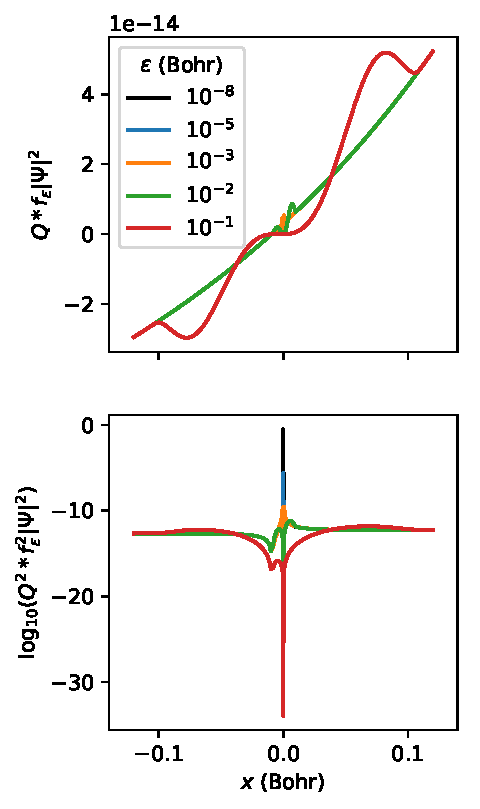
\includegraphics[width=1.0\columnwidth]{../2_plots/viznode.pdf}
\caption{$E_L\frac{\partial_p \Psi}{\Psi} f_\epsilon$ and logarithm $(E_L\frac{\partial_p \Psi}{\Psi} f_\epsilon)^2$, plotted against the normal coordinate $x$ from a node of $\Psi$. Curve colors correspond to different values of $\epsilon$ ranging from $10^{-1}$ to $10^{-8}$ Bohr.}
\end{figure}

\begin{figure}
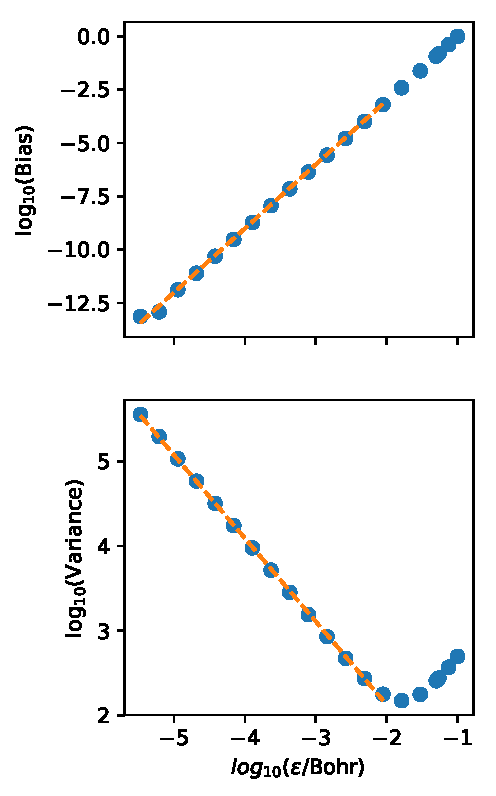
\includegraphics{../2_plots/integratenode.pdf}
\caption{Scaled bias and variance of $\frac{\hat{H}\Psi \partial_p \Psi}{\Psi^2}$ evaluated by numerical integration from $r = -0.1$ to $r = 0.1$ across the node in Figure 1. The blue dots are the numerically integrated values and the orange curves indicate best fits to the functions $a\epsilon^3$ and $b + c/\epsilon$ for the bias and variance, respectively.}
\end{figure}

\begin{figure}
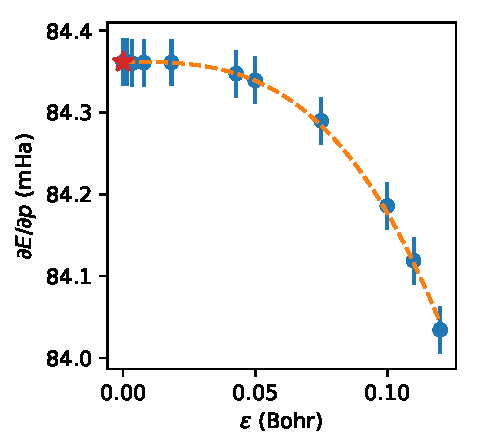
\includegraphics{../2_plots/dedp.pdf}
\caption{Zero bias, finite variance extrapolation for $\partial E/\partial p$ using the regularized estimator. The blue points are evaluated using VMC, the orange curve is a fit to $a + b\epsilon^3$, and the red star denotes the extrapolated estimation. }
\end{figure}

We begin by verifying the core claim of the regularized integrand Eqn~\ref{eq:convergent_integral} being finite across the nodes of $\Psi$ for any $\epsilon > 0$.\lucas{The integrand is not making a claim. Be more specific. Are we just verifying Eqn \ref{eq:convergent_integral}?}
To do so, we evaluate the regularized integrand for various $\epsilon$ along a path which passes through a node $\vec{N}$, $\vec{R}(x) = \vec{N} + x \nabla \Psi(\vec{N})/|\nabla \Psi(\vec{N})|$ with $x \in [-0.1, 0.1]$ Bohr.
The results are shown in the lower plot of Figure 1.
For all values of $\epsilon$, the value of the integrand is pushed to zero at the node, removing the divergence in the integral.
The sharp increase in the integrand near $x=0$ as $\epsilon$ decreases is indicative of the increase in the value of the integral, and hence estimator variance, as $\epsilon \rightarrow 0$.
Shown in the upper plot is the first term in Eqn~\ref{eq:regularized_estimator} across the node, exhibiting no divergences.

By integrating across the normal coordinate $x$, the predicted $O(1/\epsilon)$, $O(\epsilon^3)$ scalings of the variance and bias are recovered, as shown in Figure 2.
The integration for both the bias and variance are carried out for the path shown in Figure 1 from $x = -0.1$ to $0.1$ Bohr and normalized by a factor $\int |\Psi|^2 dR$ along that path.
The predicted cubic bias is observed for six decades in $\epsilon$ while the exponential decrease in variance stands for four decades.
The increase in the variance after $\epsilon = 10^{-2}$ occurs due to the breakdown of the assumption $\Psi(\vec{R}) \sim \nabla(\vec{N}) \cdot (\vec{R}-\vec{N})$, resulting in a linear increase in variance with $\epsilon$.
This change is not mirrored in the bias since the sub-leading order scaling with $\epsilon$ appears when the assumptions of $\hat{H}\Psi$ and $\partial_p \Psi \sim const$ break down.

We conclude by carrying out the four step, finite-variance extrapolation for $\partial E/\partial p$ proposed in the previous section, shown in Figure 3.
First, a standard VMC calculation with 200,000 steps and 2,000 configurations per step was carried out.
Then, $\partial E/\partial p$ was estimated using Eqn~\ref{eq:regularized_estimator} for $\epsilon$ between $10^{-1}$ Bohr and $10^{-5}$ Bohr using the VMC configurations, shown in the blue data points.
Since the same configurations were used for each evaluation, the estimates have a strong statistical correlation and the predicted $\epsilon^3$ bias is clearly present, shown by the orange fit curve.
The intercept of the fit curve is shown by the red star and is the zero-bias estimate of $\partial E/\partial p$; the variance can be deduced by the error bar of the blue data points, in this case 0.025 mHa.
Since the bias is zero within statistical errors for small values of $\epsilon$, most practical calculations can be carried out for a fixed value of $\epsilon$ between $10^{-5}$ and $10^{-2}$ Bohr without extrapolation.
\lucas{Thus the regularized estimator is quite robust to $\epsilon$}

\section{Conclusion}
Efficient estimation of $\partial E/\partial p$ is integral to the reliability of variational Monte Carlo wave function optimization methods.
Within these techniques, wave function parameters are updated iteratively, with the estimate of $\partial E/\partial p$ used in determining updates.
If the estimation is inaccurate, having a large bias, the final converged wave function is not guaranteed to be the lowest energy wave function in the parameterization space.
\lucas{it's not guaranteed anyway, unless you are doing global optimization. Need to define "parameterization space"}
If the estimation is unstable, having a large variance, the updates will have large statistical fluctuations, decreasing efficiency.
\lucas{don't use future tense here.}
While the naive Monte Carlo estimator for $\partial E/\partial p$ is unbiased, it has an infinite variance, prompting a search for finite variance estimators for the quantity.
\lucas{This paragraph is more of an introduction than a conclusion. Usually the conclusion/summary has conclusions and summaries in it.} 

In this work, we derived and tested a simple regularized estimator for $\partial E/\partial p$ which has finite variance and can be extrapolated to zero bias.
The divergent variance present in the naive Monte Carlo estimator is suppressed via multiplication by a polynomial function within a distance $\epsilon$ of the nodes of $\Psi(\vec{p}, \vec{R})$. 
We prove that the regularized estimator manages a finite variance by incurring a cubic bias which can be efficiently extrapolated to zero bias.
The extrapolation is carried out, and a finite variance, zero-bias estimate of $\partial E/\partial p$ is evaluated for a determinantal coefficient in a trial wave function for the LiH molecule.
\lucas{explain why this is advantageous and an improvement of the state of the art. }

%\bibliographystyle{unsrt}
\bibliography{pgradregr}
\end{document}